\section*{Regularization}
\color{black}
\textit{To lower generalization error but not the training error.\\
$\bullet$ informed regularization (prior knowledge)\\
$\bullet$ simplicity bias (Occam's razor)\\
$\bullet$ Bayesian averaging (ensembling, dropout)
}
\subsection*{$L_2$-Regularization / Weight Decay}

Regularized objective becomes 
$\overline{E}_\theta(S)=E_\theta(S)+\mu\Omega(\theta)$
where $\Omega(\theta) = \frac{1}{2} \sum_{l=1}^L ||W^l||_F^2 = \frac{1}{2} \sum_i \theta_i^2$ (no bias reg.) for $\theta = vec(W^1, \ldots, W^L, b^1, \ldots, b^L)$. Since $\nabla_\theta \Omega(\theta) =\mu\theta$ the GD\\ update includes weight decay: $\theta_{t+1} \!=\! (1\text{-}\eta \mu) \theta_t \text{-} \eta \nabla_\theta E_{\theta_t}$

\resizebox{\linewidth}{!}{\textbf{Spectral Analysis based on Taylor around \(\arg\min E_\theta(S)\):}}\\
$\bar E_\theta(S) \approx E_{\theta^*}(S)+\frac{1}{2}(\theta-\theta^*)^TH_E(\theta-\theta^*) + \mu \Omega(\theta) + \mathcal{O}(||\theta - \theta^*||_2^3)$ with Hessian $H_E=Q\text{diag}(\lambda_i)Q'$. By first order conditions\\ $\theta\overset{!}{=}(H_E+\mu I)^{-1}H_E\theta^*=Q\text{diag}(\frac{\lambda_i}{\lambda_i+\mu})Q'\theta^*$. Hence, along low-curvature directions ($\lambda_i \ll \mu$) the weights are shrunk.

\textbf{Constrained Optimization:}\\
Regularization objective becomes $\arg\min_{\{\theta:\norm{\theta}\leq r\}}E(\theta)$. Regularization only effective at late stages of learning.\\
Optimized using projected gradient descent:

\hspace{4pt} $\theta_{t+1}=\Pi_r[\theta_t-\eta\nabla E_{\theta_t}(S)]$ where $\Pi_r(v)=\min\left\{1,\frac{r}{\norm{v}}\right\}v$

\textbf{Ridge Regression: }Linear regression + $L_2$-regularization is termed Ridge regression with $\pmb\theta^* = (\mathbf{X}^{\intercal}\mathbf{X}+\lambda\mathrm{I})^{-1}\mathbf{X}^{\intercal}\mathbf{y}$.

\subsection*{Early Stopping}
Stop learning when loss on validation data increases. Early stopping acts as an approximate $L2$-regularizer:

\resizebox{\linewidth}{!}{\textbf{Spectral Analysis based on Taylor around \(\arg\min E_\theta(S)\):}}\\
$\nabla_\theta E_\theta(S) \approx H_E(\theta-\theta^*) + \mathcal{O}(||\theta - \theta^*||_2^2)$ w. $H_E=Q\text{diag}(\lambda_i)Q'$ giving GD update $\theta_{t+1} = \theta_t - \eta H_E(\theta_t-\theta^*) + \mathcal{O}(||\theta_t - \theta^*||_2^2$.

Hence, $\theta_{t+1} - \theta^* = (I - \eta H_E)(\theta_t-\theta^*) + \mathcal{O}(||\theta_t - \theta^*||_2^2$. Then

$\theta_t = \cancel{(I - \eta \text{diag}(\lambda_i))^t Q' \theta_0} + Q[I - (I - \eta \text{diag}(\lambda_i))^t]Q' \theta^*$

(by induction) where the first term is neglected if $\theta_0 = 0$.

Since $t \eta \text{diag}(\lambda_i) \overset{\eta \lambda_i \ll 1}{\approx} I - (I-\eta \text{diag}(\lambda_i))^t \overset{!}{=} \text{diag}(\frac{\lambda_i}{\lambda_i + \mu})$ we get $L_2$-regularization given $\eta\lambda_i \ll 1$, \underline{$\lambda_i \ll \mu$, $t=\frac{1}{\eta\mu}$}.
\subsection*{Residual Connections}
Parametrize $G_\theta(x)=x+F_\theta(x)$ with $F \approx 0$ at initialization giving Jacobian $J_G \approx I$ (good for backpropagation) and allowing weight decay toward identity. ResNets augment deep CNNs with residual connections. DenseNets further employ skip connections to all downstream layers. \\[3pt]
$\bullet$ Residual Connections adds shortcut to output\\
$\bullet$ Skip Connections concatenates shortcut to output 
\subsection*{Normalization}
Calibrate dynamic range of unit $j$ in layer $l$ (datapoint $i$):\\
\textbf{Batch Normalization ($\gamma_j^l, \beta_j^l$ are params):}\\
Normalization: $\Tilde{z}_j^l[i]=\frac{z_j^l[i]-\mu_j^l}{\sigma_j^l+ \delta} \quad 0 < \delta \approx 0, \hfill \hat{z}_j^l=\gamma_j^l+\beta_j^l\Tilde{z}_j^l$\\
Statistics: $\mu_j^l = \frac{1}{|B|} \sum_{i \in B} z_j^l [i], \hfill (\sigma_j^l)^2 = \frac{1}{|B|} \sum_{i \in B} (z_j^l [i] - \mu_j^l)^2$\\
\textbf{Layer Normalization (normal. along single instance):}\\[5pt]
Normalization:  \underline{same formula as in Batch Norm}\\[5pt]
Statistics: $\mu_j^l = \frac{1}{m_l} \sum_{j =1}^{m_l} z_j^l [i], \hfill (\sigma_j^l)^2 = \frac{1}{m_l} \sum_{j =1}^{m_l} (z_j^l [i] - \mu_j^l)^2$\\
\subsection*{Dropout}
Randomly drop subsets of units for more robustness with retention probability $\pi_i^l$ for unit $i$ in layer $l$ (input $\pi_i^0=0.8$ and hidden unit $\pi_i^{l\geq 1}=0.5$). Creates an 
\underline{exponentially large (in \#nodes) ensemble} of networks.\\[5pt]
At inference, use as an ensemble method or rescale weights $\Tilde{w}_{ij}^l\leftarrow\pi_j^{l-1}w_{ij}^l$ calibrating the net input to unit $i$.
\subsection*{Data Augmentation}
\textit{Trick to generate larger, non-i.i.d. training set}\\[5pt]
Generate virtual examples by applying transformations $\tau$ to each training example $(\mathbf{x},\mathbf{y})\mapsto (\tau(\mathbf{x}),\mathbf{y})$, e.g. 
PCA, cropping \& resizing, rotations \& reflections, etc.\\[5pt]
We can add noise to the inputs (ideally realistic noise), to the weights (regularizing effect) or to the targets (soft targets/label errors). Also helps with model robustness. 
\subsection*{Self-Supervised Training}
Pretrain a model on a (self-supervised) task (e.g. patch location prediction, image coloring, video motion prediction, predictive coding of latent states) before finetuning.\\[5pt]
\textbf{Contrastive Predictive Coding}

\begin{minipage}{.6\linewidth}
    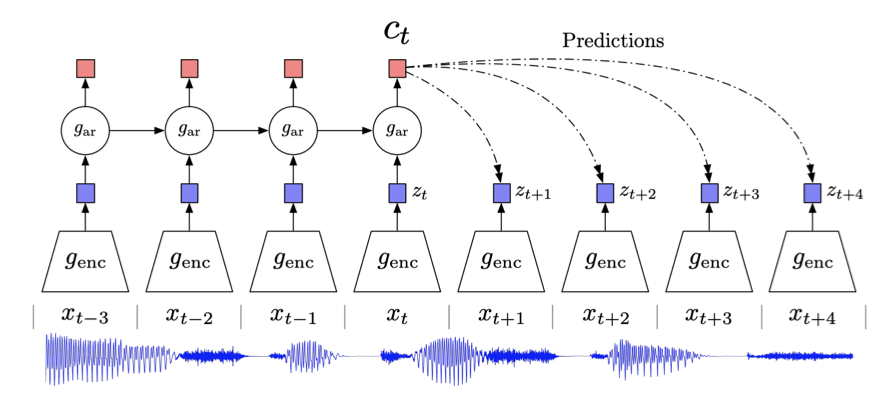
\includegraphics[width=\linewidth]{contrastive_predictive_coding.png}
\end{minipage}
\begin{minipage}{.4\linewidth}
    Maxim. density ratio\\
    $\frac{p(x_{t+1}\mid c_t)}{p(x_{t+1})} \propto e^{z_{t+1}^TWc_t}$\\
    for positive examples\\ and minimize for\\
    negative examples
\end{minipage}
